\documentclass{../sftex/sftex}

\usepackage[portuguese, onelanguage]{algorithm2e}
\usepackage{amsmath, amsfonts, enumitem, tikz, parskip, url}

\newcommand{\hh}{$\mathcal{H}$}
\newcommand{\pk}{$\mathcal{P}_k$}
\newcommand{\sk}{$\mathcal{S}_k$}
\newcommand{\hash}[2][]{\mathcal{H}^{#1} (#2)}
\newcommand{\concat}{\, \vert{} \vert{} \,}
\newcommand{\binwds}[1]{\{0, 1\}^{#1}}
\newcommand{\length}[1]{\vert{} #1 \vert{}}

\renewcommand*{\thefootnote}{(\arabic{footnote})}

\title{Esquemas de assinatura digital pós-quânticos \\ baseados em AES}
\author{Gustavo Zambonin, Marcello da Silva Klingelfus Junior}
\email{\{gustavo.zambonin,marcello.klingelfus\}@grad.ufsc.br}
\src{https://github.com/zambonin/epos-aes-docs}
\uniclass{Sistemas Operacionais II}
\classcode{UFSC-INE5424}

\begin{document}

\maketitle

\section{Introdução}

{\footnotesize Texto parcialmente reproduzido do Trabalho de Conclusão de Curso
do primeiro autor.}

A aplicação de protocolos criptográficos é essencial no contexto da validação e
proteção de quaisquer comunicações realizadas por um conjunto de entidades,
sejam estas dispositivos eletrônicos ou indivíduos, em virtude da possível
criticalidade e sensibilidade atribuídas aos dados transmitidos. Esquemas de
assinatura digital são comumente utilizados para assegurar este processo de
maneira formal~\cite{Goldreich:2004:FCV:975541}, através da autenticidade e
não-repúdio do remetente e certeza da integridade dos dados, a fim de
traduzir o resguardo provido por uma assinatura de próprio punho no mundo real.

Na prática, a maior parte destes esquemas utilizam como alicerce algorítmico
criptossistemas assimétricos baseados em problemas ``difíceis'' da teoria dos
números, como a fatoração de inteiros ou resolução do logaritmo discreto, ambos
para números grandes. Este fato provê a segurança necessária para os esquemas
em computadores clássicos (eletrônicos), por conta da inexistência de
algoritmos que resolvem estes problemas em tempo polinomial, até o momento.
Entretanto, em computadores quânticos, algoritmos dessa forma já existem --- em
especial, o algoritmo de Shor~\cite{Shor:1997:PAP:264393.264406} ---
efetivamente tornando estes esquemas clássicos inseguros neste novo contexto.

Para combater esta situação, a criptografia pós-quântica encarrega-se de buscar
algoritmos criptográficos cuja segurança é considerada suficiente mesmo
utilizando-se de um computador quântico e ataques especializados, como o
algoritmo de Grover~\cite{Grover:1996:FQM:237814.237866}. Esta área conta com
diversas abordagens diferentes: a criptografia baseada em reticulados,
polinômios multivariados sobre um corpo finito, códigos de correção de erros,
morfismos entre curvas elípticas supersingulares, criptossistemas simétricos
e funções de resumo criptográfico. Em especial, é possível mesclar as duas
últimas opções a fim de aproveitar, respectivamente, o desempenho e a
simplicidade destas, bem como demonstrar a versatilidade garantida pelas
diferentes funções que podem ser utilizadas para a criação destes esquemas.

\section{Funções de resumo criptográfico}

Uma função de resumo \hh{} mapeia valores deterministicamente entre dois
conjuntos. O domínio pode ter tamanho infinito, e neste caso a função pode ser
chamada de função de compressão; a imagem deve ser estritamente menor do que o
domínio e finita, e elementos deste conjunto são chamados de resumos. É
desejável para \hh{} que estes mapeamentos ocorram de tal maneira que não
ocorra uma relação aparente entre entradas e saídas da função. Funções de
resumo adicionadas de propriedades que tornam-as adequadas para utilização no
contexto de segurança da informação são chamadas de funções de resumo
criptográfico, e possibilitam a certeza da integridade de dados, mesmo que
armazenados em um dispositivo inseguro.

Tome $X : \binwds{*}$ e $Y : \binwds{n}$, $n \in \mathbb{N}$. Então,
$\mathcal{H} : X \longrightarrow Y$. De acordo
com~\cite{stinson2005cryptography}, para que qualquer \hh{} seja considerada
criptográfica, deve ser difícil resolver os três problemas listados abaixo.  É
importante notar que um problema é considerado ``difícil'', ou
computacionalmente impraticável, quando o tempo ou recursos gastos para esta
computação excedem a validade ou utilidade da informação desejada.

\begin{enumerate}[label=\roman*.]

  \item Fornecido um resumo $h \in Y$, achar a mensagem original $m \in X$ que
    gerou $h$ através de $\hash{m} = h$; \hh{} é considerada resistente à
    pré-imagem (\textsc{Pre}) se isto não pode ser resolvido de maneira
    eficiente.

  \item Fornecida uma mensagem $m_0 \in X$, achar uma mensagem $m_1 \in X$ tal
    que $m_0 \neq m_1$ e $\hash{m_0} = \hash{m_1}$. \hh{} é considerada
    resistente à segunda pré-imagem (\textsc{Sec}) se isto não pode ser
    resolvido de maneira eficiente.

  \item Para quaisquer duas mensagens $m_0, \; m_1 \in X$ e $m_0 \neq m_1$,
    $\hash{m_0} = \hash{m_1}$. \hh{} é considerada resistente à colisões
    (\textsc{Col}) se isto não pode ser resolvido de maneira eficiente.

\end{enumerate}

\section{AES --- \emph{Advanced Encryption Standard}}

O AES é uma cifra de blocos que opera sobre uma matriz de estado $A$, onde
$A_{i,j} \in \mathbb{F}_{2^{8}}$\footnote{Definido pelo polinômio irredutível
$m(x) = x^{8} + x^{4} + x^{3} + x + 1$. Adições e multiplicações em corpos da
forma $\mathbb{F}_{2^n}$ são, respectivamente, representadas por operações
\texttt{AND} e \texttt{XOR}, e coeficientes de polinômios são palavras
binárias, tornando esta estrutura convidativa para operações computacionais.},
$0 \leq i, j < 4$, a partir de uma chave $K$ de tamanho $n = \{128, 192,
256\}$. É uma versão padronizada pelo NIST (\emph{National Institute of
Standards and Technology})~\cite{Standards2001} do algoritmo
Rjindael~\cite{Daemen:2002:DR:560131}. Seu funcionamento é denominado
iterativo, consistindo em aplicações sequenciais de quatro operações ordenadas
(\textsc{SubBytes}, \textsc{ShiftRows}, \textsc{MixColumns} e
\textsc{AddRoundKey}) sobre $A$. A quantidade destas aplicações, denominadas
rodadas ($n_r$), depende diretamente do tamanho da chave: $n = 128 \rightarrow
n_r = 10, n = 192 \rightarrow n_r = 12, n = 256 \rightarrow n_r = 14$.

Note que existe uma rodada adicional introdutória composta apenas de
\textsc{AddRoundKey}, para que o estado inicial seja modificado. Ademais,
\textsc{MixColumns} é ignorado na última rodada, a fim de facilitar a
reversibilidade da cifra. Uma rotina de expansão de chave
(\textsc{KeyExpansion}) existe para que $K$ seja propagada em todas as rodadas
com valores derivados, porém distintos. Estes componentes serão descritos
abaixo.

\begin{enumerate}[label=\roman*.]

    \item \textsc{SubBytes}: realiza-se a reposição de $A_{i,j}$
        pelo seu valor correspondente em uma \emph{substitution-box}
        (\emph{S-box}, construída a partir de uma transformação afim em
        $A_{i,j}^{-1}$ sobre $\mathbb{F}_2$), onde os \emph{nibbles} mais e
        menos significativos, respectivamente, representam a linha e a coluna
        do elemento na \emph{S-box}.

    \item \textsc{ShiftRows}: cada linha de $A$, $A_i$, é deslocada
        circularmente à esquerda $i$ vezes.

    \item \textsc{MixColumns}: cada coluna de $A$, $A_j$, é multiplicada pelo
        polinômio $c = 03 \cdot x^{3} + 01 \cdot x^{2} + 01 \cdot x + 02$,
        módulo $x^{4} + 1$, para que o resultado ainda seja um polinômio de
        grau máximo 3, apto a ser representado na coluna.

    \item \textsc{AddRoundKey}: a operação \texttt{XOR} bit a bit é aplicada
        entre $A$ e o bloco da chave referente à rodada.

\end{enumerate}

\textsc{KeyExpansion} consiste da criação de um conjunto de palavras $K_e$ de
32 bits.  Tome $\ell = \frac{n}{32}$, e assumindo que é necessário criar
palavras suficientes para utilização em todas as rodadas do algoritmo, então $t
= \ell \cdot (n_r + 1)$ e $K^e = \{k_0, \dots, k_{t - 1}\}$. Também defina
$rot(x)$ como o deslocamento circular à esquerda de 8 bits da palavra $x$, e a
lista de constantes $RC$ com elementos em $\mathbb{F}_{2^{8}}$ definida pela
recursão $RC_0 = x^0, RC_1 = x^1, RC_j = x^{j-1} \cdot RC_{j-1}, j > 2$.
Inicialmente, $\{k_0, \dots, k_{\ell - 1}\} = K$, e $\forall i \geq \ell,
K^{e}_{i} = K^{e}_{i - \ell} \oplus \mathbf{k}$. A palavra $\mathbf{k}$,
inicialmente com valor $K^{e}_{i - 1}$, pode ser modificada de acordo com as
restrições (mutualmente exclusivas) abaixo.

\begin{itemize}
    \item $i \equiv 0 \pmod{4} \rightarrow \mathbf{k}
        = \textsc{SubBytes}(rot(K^{e}_{i - 1})) \oplus RC_{\frac{i}{\ell}}$;
    \item $\ell = 8 \land i \equiv 4 \pmod{8} \rightarrow \mathbf{k}
        = \textsc{SubBytes}(K^{e}_{i - 1})$.
\end{itemize}

Assim, uma função que criptografa uma mensagem $m$ e retorna um texto cifrado
$c$ pode ser representada pelo pseudocódigo abaixo.

\begin{algorithm}[H]
    \KwData{$m$, o texto a ser cifrado; $K$, a chave desejada}
    \KwResult{$c$, o texto cifrado resultante}

    $A \longleftarrow m$\;
    $K^{e}_{0} \dots K^{e}_{(n_r + 1) \cdot \ell}
        \longleftarrow \textsc{KeyExpansion}(K)$\;
    $A \longleftarrow \textsc{AddRoundKey}(A,
        \{K^{e}_{0}, \dots, K^{e}_{\ell - 1}\})$\;

    \For{$i \leftarrow 1$ \KwTo{} $n_r - 1$}{
        $A \longleftarrow \textsc{SubBytes}(A)$\;
        $A \longleftarrow \textsc{ShiftRows}(A)$\;
        $A \longleftarrow \textsc{MixColumns}(A)$\;
        $A \longleftarrow \textsc{AddRoundKey}(A,
            \{K^{e}_{i \cdot \ell}, \dots, K^{e}_{(i + 1) \cdot \ell - 1}\})$\;
    }

    $A \longleftarrow \textsc{SuhbBytes}(A)$\;
    $A \longleftarrow \textsc{ShiftRows}(A)$\;
    $A \longleftarrow \textsc{AddRoundKey}(A,
        \{K^{e}_{n_r \cdot \ell}, \dots, K^{e}_{(n_r + 1) \cdot \ell - 1}\})$\;

    $c \longleftarrow A$\;
\end{algorithm}

Para que a cifra seja caracterizada como simétrica, é preciso criar uma função
que faça o inverso do procedimento acima. Assim, suas etapas precisam ser
modificadas de acordo.

\begin{enumerate}[label=\roman*.]

    \item \textsc{InvShiftRows}: cada linha de $A$, $A_i$, é deslocada
        circularmente à direita $i$ vezes.

    \item \textsc{InvSubBytes}: é necessário computar a transformação afim
        inversa para cada elemento $A_{i,j}$, e depois calcular sua inversa
        multiplicativa.

    \item \textsc{InvMixColumns}: cada coluna de $A$, $A_j$, é multiplicada
        pela inversa multiplicativa $d = c^{-1}$, obtida por: $(03 \cdot x^{3}
        + 01 \cdot x^{2} + 01 \cdot x + 02) \cdot d \equiv 1 \pmod{x^{4} + 1}$,
        logo $d(x) = 0B \cdot x^{3} + OD \cdot x^{2} + 09 \cdot x + 0E$.

\end{enumerate}

Por fim, o algoritmo resultante pode ser representado pelo pseudocódigo abaixo.
Note a mudança da ordem das etapas, e a utilização invertida de $K_e$.

\begin{algorithm}[H]
    \KwData{$c$, o texto cifrado; $K$, a chave desejada}
    \KwResult{$m$, o texto claro resultante}

    $A \longleftarrow c$\;
    $K^{e}_{0} \dots K^{e}_{(n_r + 1) \cdot \ell}
        \longleftarrow \textsc{KeyExpansion}(K)$\;
    $A \longleftarrow \textsc{AddRoundKey}(A,
        \{K^{e}_{n_r \cdot \ell}, \dots, K^{e}_{(n_r + 1) \cdot \ell - 1}\})$\;

    \For{$i \leftarrow n_r - 1$ \KwTo{} $1$}{
        $A \longleftarrow \textsc{InvShiftRows}(A)$\;
        $A \longleftarrow \textsc{InvSubBytes}(A)$\;
        $A \longleftarrow \textsc{AddRoundKey}(A,
            \{K^{e}_{i \cdot \ell}, \dots, K^{e}_{(i + 1) \cdot \ell - 1}\})$\;
        $A \longleftarrow \textsc{InvMixColumns}(A)$\;
    }

    $A \longleftarrow \textsc{InvShiftRows}(A)$\;
    $A \longleftarrow \textsc{InvSubBytes}(A)$\;
    $A \longleftarrow \textsc{AddRoundKey}(A,
        \{K^{e}_{0}, \dots, K^{e}_{\ell - 1}\})$\;

    $m \longleftarrow A$\;
\end{algorithm}

\section{Criptografia simétrica}

Algoritmos criptográficos que utilizam a mesma chave para criptografar o
texto plano e descriptografar o texto correspondente cifrado são classificados
como algoritmos de criptografia simétrica. A chave representa um segredo
compartilhado entre entidades em uma comunicação segura. Porém, a necessidade
de um canal seguro para o estabelecimento desta chave apresenta-se como uma
desvantagem deste tipo de criptografia. Geralmente, cifras de bloco (DES, AES)
ou de fluxo (RC4, Salsa20) são a base para estes algoritmos. Utilizando estas
como alicerce, é possível construir funções de resumo criptográfico: por
exemplo, a construção Merkle-Damgård, base para as funções MD5, SHA1 e SHA2,
utiliza uma função de compressão única, obtida a partir de uma cifra de
bloco~\cite[9.14]{Menezes:1996:HAC:548089}.

\section{Criptografia assimétrica}

Em contrapartida, a criptografia assimétrica, ou criptografia de chaves
públicas, engloba os algoritmos que utilizam um par de chaves: a chave privada
(\sk{}), conhecida apenas pela entidade que a gerou, e a chave pública (\pk{}),
distribuída livremente. Isto possibilita o uso livre de \pk{} para a
comunicação segura com o detentor da chave sem a necessidade de um canal
seguro, em virtude da construção dos algoritmos. A segurança destes depende da
``dificuldade'' computacional de determinar uma chave privada a partir da chave
pública, e também do armazenamento de \sk{} em um lugar seguro. Problemas em
teoria de números e álgebra que atualmente não admitem soluções em tempo
polinomial são comumente utilizados como base para algoritmos assimétricos.
Porém, percebe-se que, com a introdução de um computador quântico, estes
problemas podem ser resolvidos de maneira significativamente mais rápida, como
visto em~\cite{Shor:1997:PAP:264393.264406}.

\section{Esquemas de assinatura digital}

Um esquema de assinatura digital é uma construção matemática que habilita a
demonstração de certas propriedades sobre mensagens assinadas: nomeadamente, a
autenticação do remetente, onde esta entidade pode ser facilmente identificada
como a emissora da assinatura digital; a integridade da mensagem, \emph{i.e.} a
certeza de que esta não foi modificada ao ser transmitida por um canal
possivelmente inseguro; e o não-repúdio do remetente, onde não é possível negar
que uma mensagem foi assinada e enviada, após este fato.

\begin{figure}[h]
  \centering
  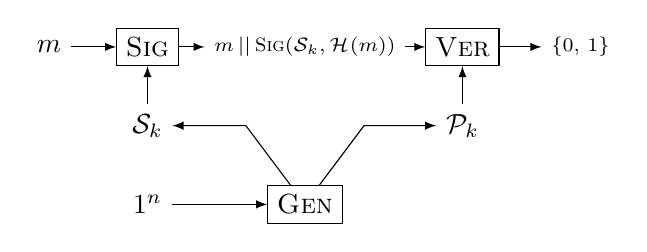
\begin{tikzpicture}
    \node (hm) at (-1.25, 0) {$m$};
    \node (in) at (0, -2) {$1^n$};
    \node (sk) at (0, -1) {\sk{}};
    \node (pk) at (4, -1) {\pk{}};
    \node (ds) at (2, 0)
      {\scriptsize{$m \concat \textsc{Sig}(\text{\sk{}}, \hash{m})$}};
    \node (res) at (5.5, 0) {\scriptsize\{0, 1\}};
    \node[draw] (sig) at (0, 0) {\textsc{Sig}};
    \node[draw] (gen) at (2, -2) {\textsc{Gen}};
    \node[draw] (ver) at (4, 0) {\textsc{Ver}};
    \draw[-latex] (gen) to (1.25, -1) to (sk);
    \draw[-latex] (gen) to (2.75, -1) to (pk);
    \draw[-latex] (sk) -- (sig);
    \draw[-latex] (hm) -- (sig);
    \draw[-latex] (sig) -- (ds);
    \draw[-latex] (ds) -- (ver);
    \draw[-latex] (pk) -- (ver);
    \draw[-latex] (ver) -- (res);
    \draw[-latex] (in) -- (gen);
  \end{tikzpicture}
  \caption{Funcionamento típico de um
    esquema de assinatura digital.}\label{fig:2}
\end{figure}

Esquemas de assinatura digital são fortemente baseados em criptografia de
chaves públicas, e consistem de três algoritmos: a geração de chaves
$\textsc{Gen}(1^n)$, que gera um par de chaves aleatório (\pk{},
 \sk{}) com parâmetro de segurança $n$; o algoritmo de assinatura
$\textsc{Sig}(\text{\sk{}}, m)$, que produz uma assinatura $\sigma$ para uma
mensagem $m$; e o algoritmo de verificação $\textsc{Ver}(\text{\pk{}}, m,
\sigma)$, que retorna o estado de validade da assinatura como um valor verdade
binário. De acordo com~\cite{Goldreich:2004:FCV:975541}, todas as assinaturas
geradas por \textsc{Sig} devem ser verificáveis por \textsc{Ver} utilizando
todas as chaves geradas por \textsc{Gen}. Formalmente, $\forall (p, s) \in
\textsc{Gen}^{\rightarrow}(1^n)$ e $\forall w \in \binwds{*}$,
\begin{equation}
    \text{Pr}[\textsc{Ver}(p, w, \textsc{Sig}(s, w)) = 1] = 1.
\end{equation}
Na Figura~\ref{fig:2}, é possível visualizar um diagrama do comportamento de
um esquema de assinatura digital genérico. Note que $\sigma$ geralmente é
composto da concatenação da mensagem original com a assinatura do resumo
criptográfico desta, embora a saída do algoritmo \textsc{Sig} consista apenas
da aplicação de uma função interna a este ao resumo.

\section{O esquema Winternitz}

O esquema de assinatura digital única Winternitz (\textsc{Wots} ---
\emph{Winternitz one-time signature}), em sua proposta
original~\cite{Merkle:1989:CDS:118209.118230}, apresenta versatilidade em
relação ao tamanho de chaves e da assinatura, e também pode ser configurado
para utilizar diferentes funções de resumo criptográfico a fim de utilizar
recursos possivelmente disponíveis no dispositivo alvo.

Tome um parâmetro de segurança $m$, geralmente considerado como o tamanho da
saída da função de resumo criptográfico escolhido. Um parâmetro $w \in
\mathbb{N}, w > 1$ também deve ser definido, responsável por codificar a
quantidade de bits a serem assinados simultaneamente, modificando assim o
desempenho geral do esquema e o tamanho de chaves e assinatura. A partir
destes, calcula-se
    \[t_1 = \left\lceil \frac{m}{w} \right\rceil, \; t_2 = \left\lceil
    \frac{\left\lfloor \log_2 t_1 \right\rfloor + 1 + w}{w} \right\rceil
    \text{ e } t = t_1 + t_2.\]
Por fim, considere as funções\footnote{Na prática, o esquema pode ser
instanciado utilizando \hh{} no lugar de $f$.} de mão única $f : \binwds{m}
\longrightarrow \binwds{m}$ e de resumo criptográfico $\mathcal{H} : \binwds{*}
\longrightarrow \binwds{m}$.  Descreve-se abaixo o funcionamento do esquema e
discute-se algumas de suas características.

\begin{enumerate}

    \item[] \emph{Geração de chaves.} Defina $\text{\sk{}} = (x_{t-1}, \dots,
        x_0) \stackrel{\$}{\longleftarrow} \binwds{m}$ como a chave privada,
        informalmente uma $t$-tupla de inteiros pseudoaleatórios. A chave
        pública $\text{\pk{}} = (y_{t-1}, \dots, y_0)$ pode ser derivada de
        \sk{}, computando $f^{2^{w}-1}(x) \; \forall x \in  \text{\sk{}}$.
        Logo, $\text{\pk{}} = (f^{2^{w}-1}(x_{t-1}), \dots, f^{2^{w}-1}(x_0))$.

    \item[] \emph{Geração da assinatura.} Tome uma mensagem $M$ e calcule o seu
        resumo $d = \mathcal{H}(M)$. Por conveniência, escolhe-se $m$ ou $w$ de
        forma que $w \mid m$, mas podem ser concatenados zeros ao resumo para
        que isso seja satisfeito. $d$ é dividido em uma $t_1$-tupla de palavras
        em base-$w$, $\mathcal{B}_1 = (b_{t-1}, \dots, b_{t-t_1})$.
        Adicionalmente, uma soma de verificação é calculada usando a
        representação inteira dos elementos de $\mathcal{B}_1$: $c = \sum_{b
        \in \mathcal{B}_1} 2^w - 1 - b$. Novamente, $c$ pode ser arredondado
        com zeros até que $w \mid \length{c}$. Finalmente, $c$ é dividido em
        uma $t_2$-tupla de palavras base-$w$, $\mathcal{B}_2 = (b_{t_2-1},
        \dots, b_0)$. Assim, $\mathcal{B} = \mathcal{B}_1 \cup \mathcal{B}_2$ e
        obtém-se a assinatura $\sigma = (f^{b_{t-1}}(x_{t-1}), \dots,
        f^{b_0}(x_0))$.

    \item[] \emph{Verificação da assinatura.} Para assegurar a corretude da
        assinatura $\sigma$, todos os blocos $\sigma_i$ precisam ser
        verificados separadamente através do cálculo das aplicações restantes
        de $f$. Assim, computando $\mathcal{B}$ novamente, $\sigma$ está
        correta se $\text{\pk{}} = (f^{2^w - 1 - b_{t-1}}(\sigma_{t-1}), \dots,
        f^{2^w - 1 - b_0}(\sigma_0))$.

\end{enumerate}

Note que não é possível decrementar valores $b_i \in \mathcal{B}$, pois isto
implicaria em achar uma pré-imagem de $f$, o que é computacionalmente inviável
em vista da restrição para $f$. Então, resta apenas a tentativa da falsificação
de $\sigma$ incrementando algum valor $b_i$. A soma de verificação $c$ é
necessária a fim de proteger o esquema contra este comportamento. Observe que,
em sua ausência, é possível que uma entidade maliciosa crie assinaturas
$\sigma'$ apenas calculando mais iterações de $f$ em blocos da assinatura
$\sigma$. Entretanto, com a presença de $c$, e consequentemente
$\mathcal{B}_2$, ao modificar um valor $b_j \in \mathcal{B}_1$, para que o
valor correto de $\mathcal{B}_2$ seja mantido, é necessário que uma pré-imagem
de algum bloco $b_k \in \mathcal{B}_2$ seja calculada. Analogamente, modificar
algum valor de $\mathcal{B}_2$ também tornará a verificação da assinatura
impossível.

\subsection{\textsc{Wots+}}

O principal esquema variante do \textsc{Wots}, chamado de
\textsc{Wots+}~\cite{cryptoeprint:2017:965}, tem como ideia principal a
reposição de $f$ por uma família de funções $\mathcal{F}_k$, substituindo o
processo de iterações sequenciais --- utilizando apenas uma função --- do
esquema original. Esta característica também permite uma prova de segurança
mais simples, mas não menos poderosa, que desconsidera a necessidade da
resistência à colisões de $f$.

Defina os parâmetros $m, w$ e a partir destes, $t_1, t_2 \text{ e } t$, bem
como a função de resumo criptográfico $\mathcal{H} : \binwds{*} \longrightarrow
\binwds{m}$ de maneira análoga ao esquema original. A família de funções que o
\textsc{Wots+} utiliza é definida por $\mathcal{F}_k : \{f_k : \binwds{m}
\longrightarrow \binwds{m} \mid k \in \mathcal{K}_m\}$, ou seja, funções de mão
única sem compressão, e $\mathcal{K}_n$ é interpretado como o espaço de chaves.
A partir desta família, e de uma tupla de palavras pseudoaleatórias $r = (r_0,
\dots, r_{2^w - 1}) \stackrel{\$}{\longleftarrow} \binwds{m}$, elabora-se a
nova função de iteração $c^{i}_{k}(x, r)$, definida recursivamente como
$c^{0}_{k}(x, r) = x, \; c^{i}_{k}(x, r) = f_k(c^{i-1}_{k}(x, r) \oplus r_i)$.

\begin{enumerate}

    \item[] \emph{Geração de chaves.} Defina \sk{} e $r$ como tuplas de
        inteiros pseudoaleatórios, discutidos anteriormente. O algoritmo também
        deve escolher uma chave de função $k \stackrel{\$}\longleftarrow
        \mathcal{K}$. Por fim, $\text{\pk{}} = (c^{2^w-1}_{k}(x_{t-1}, r),
        \dots, c^{0}_{k}(x, r))$.

    \item[] \emph{Geração da assinatura.} Tome uma mensagem $M$, calcule o seu
        resumo $d = \mathcal{H}(M)$ e a soma de verificação $c$ correspondente,
        produzindo $\mathcal{B}$. As considerações sobre preenchimento de $m$ e
        $c$ ainda se aplicam. Aplicando a nova função de iteração, tem-se
        $\sigma = (c^{b_{t - 1}}_{k}(x_{t-1}, r), \dots, c^{b_{0}}_{k}(x_{0},
        r))$.

    \item[] \emph{Verificação da assinatura.} Novamente, é necessário calcular
        $\mathcal{B}$ para obter as iterações restantes até \pk{}. Assim,
        $\sigma$ está correta se $\text{\pk{}} = (c^{2^{w} - 1 - b_{t -
        1}}_{k}(\sigma_{t-1}, r), \dots, c^{2^{w} - 1 - b_{0}}_{k}(\sigma_{0},
        r))$. Note que as primeiras $b_i$ palavras de $r$ não serão utilizadas.

\end{enumerate}

Note que é possível utilizar uma função conhecida, como o AES, para as
iterações de $f$. Isto pode ser explicado por conta de implementações em
hardware de rotinas relacionadas, como o conjunto de instruções AES-NI da
Intel, habilitando um grande ganho de desempenho no cômputo desta cifra. Porém,
é necessário adaptar a cifra de blocos para que respeite as restrições impostas
pelo esquema \textsc{Wots+}. Para que isto seja feito de maneira a manter um
nível de segurança suficiente, é possível empregar a construção
Matyas-Meyer-Oseas (MMO,~\cite[9.41]{Menezes:1996:HAC:548089}).

Assuma uma cifra de blocos genérica $E_{k}$ parametrizada pela chave $k$, cujo
bloco tem um tamanho de $n$ bits. Tome um vetor de inicialização $IV$ de
tamanho $n$, e uma função $g$ que adapte sua entrada para chaves do tamanho
necessário por $E_{k}$. Deseja-se obter um resumo $h_k$ de tamanho $n$ que
represente uma palavra $x$, e que sua inversibilidade seja computacionalmente
inviável. Deste modo, $X = (x_0, \dots, x_{k - 1}), \forall x_i \in X, \vert
x_i \vert = n$, ou seja, divida $x$ em uma $t$-tupla cujos elementos têm
tamanho $n$ --- preenchimento com zeros pode ser aplicado caso existam
elementos que desrespeitem esta regra. O resultado deste processo é definido
recursivamente como $h_0 = IV, h_i = E_{g(h_{i-1})}(x_i) \oplus x_i, 1 \leq i
\leq t$.

Utilizando este método, é possível integrar AES junto ao \textsc{Wots+}, como
forma de executar iterações para criar e verificar a assinatura, como sugerido
por~\cite[4.1]{cryptoeprint:2017:965}. Note que apenas esta versão do esquema
pode beneficiar-se deste método, em virtude dos elementos pseudoaleatórios $r$
aplicados em cada iteração. Do contrário, o método pode introduzir
multicolisões em \textsc{Wots}, efetivamente reduzindo sua segurança total.

\subsection{Esquemas baseados em árvores de Merkle}

A criação de um par de chaves para cada mensagem, bem como a infraestrutura
necessária para relacionar múltiplas chaves a uma entidade, podem tornar-se
processos extremamente onerosos. Desse modo, assim como esquemas de assinatura
digital clássicos, deseja-se que uma chave privada possa assinar múltiplos
documentos. No contexto de esquemas baseados em funções de resumo
criptográfico, a estrutura de dados chamada de árvore de Merkle, geralmente de
característica binária e perfeita, pode ser aproveitada para tal.

De modo genérico, folhas de uma árvore de Merkle são construídas a partir do
resumo criptográfico de dados que desejam ser inseridos nesta. Então, pais
destas folhas computarão o resumo criptográfico do valor dos resumos de seus
filhos concatenados, repetindo este processo até que a raiz seja preenchida.
Esta estrutura também pode ser utilizada para verificação conjunta da
integridade de múltiplos arquivos, visto que qualquer mudança em um nó da
árvore produzirá um valor distinto na raiz quando calculado novamente,
descaracterizando a validade dos dados atrelados a esta.

O primeiro esquema de assinatura digital baseado em árvores de
Merkle~\cite{Merkle:1989:CDS:118209.118230} habilita a assinatura de até
$2^{20}$ mensagens. Informalmente, os dados inseridos em suas folhas são chaves
públicas de diferentes instâncias de um esquema de assinatura única, como
\textsc{Wots}.  Assim, ao construir a árvore de Merkle, a raiz será a chave
pública deste esquema, que validará todas as folhas da árvore através de um
caminho de autenticação. A chave privada pode ser descrita como o conjunto de
chaves privadas das folhas. Vários outros esquemas continuam utilizando
assinatura única e compõem o estado da arte da
literatura~\cite{sphincsplus,irtf-cfrg-xmss-hash-based-signatures-12},
demonstrando a utilidade destes esquemas e suas otimizações.

\bibliographystyle{alpha}
\bibliography{report}

\end{document}
